\begin{figure*}
    \centering
    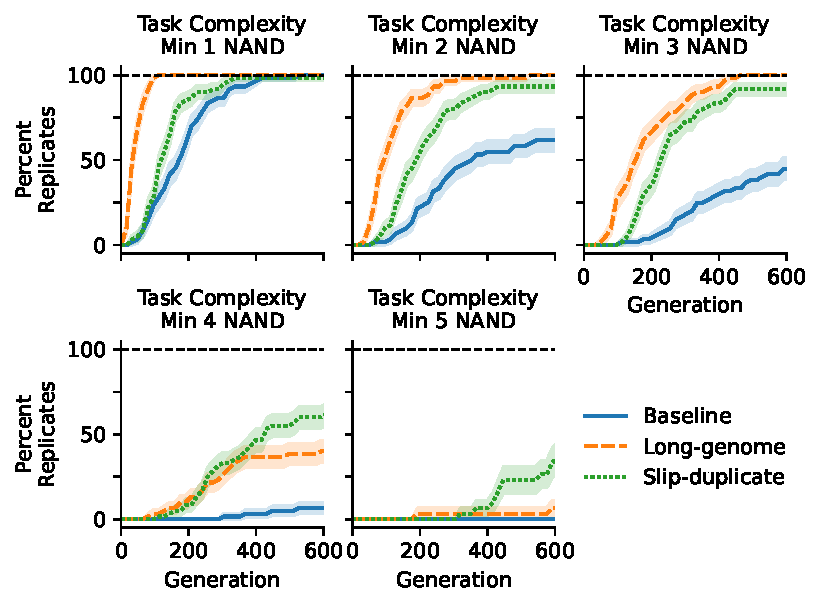
\includegraphics[width=\linewidth]{binder/binder/teeplots/adaptive-evolution-rate.ipynb/col=task-complexity+errorbar=se+hue=treatment+kind=line+mutation=per site+post=plt-xlim-0-600+style=treatment+viz=relplot+x=generation+y=has-task+ext=.pdf}
    \caption{
        \textbf{Gene duplication boosts adaptive evolution of complex phenotypic traits.}
        \footnotesize
        Plots show fraction of replicates exhibiting available phenotypic traits, by generation from founding ancestor.
        Panels facet by trait complexity, measured by the minimum number of NAND operations required to complete the task.
        Simple tasks (top left) require only one NAND operation.
        More complex tasks require up to five NAND operations (bottom right).
        Slip-duplication treatment facilitates significantly faster adaptive evolution than long-genome treatment for more complex tasks, requiring 4 or 5 components.
        Error bands give 95\% CI, bootstrapped over 30 replicates per treatment.
    }
    \label{fig:adaptive-evolution-rate}
\end{figure*}
